\section{Datos y protocolo experimental}\label{sec:datos}

\subsection{Cohorte auditada, depuración causal y hallazgos exploratorios}

La base empírica integra cuatro fuentes de información entre el 1 de enero de 2024 y el 31 de octubre de 2026 ($1\,035$ días calendario): (1) generación horaria real y capacidad efectiva neta diaria reportadas por el operador del mercado eléctrico colombiano XM \cite{xm2026api}; (2) coordenadas verificadas de centrales en el \textit{Global Solar Power Tracker} \cite{gem2026solar}; (3) pronósticos meteorológicos horarios $D+1$ archivados con $24\text{ h}$ de antelación (promedio de ECMWF IFS $0{,}25^\circ$, GFS e ICON) mediante la API \textit{Previous Runs} de Open-Meteo \cite{openmeteoPreviousRuns}; y (4) corridas operacionales subestacionales NOAA GEFSv12 (\texttt{00~UTC}, pasos hasta $696\text{ h}$) con $65\,688$ registros completos planta--origen--horizonte. Durante la auditoría de datos se descartó expresamente reconstruir series históricas $D+1$ con las primeras horas de cada corrida meteorológica, pues su proximidad al reanálisis (correlación $0{,}976$ frente a $0{,}615$ del pronóstico real a un día) habría introducido fuga futura.

El protocolo de depuración física \cite{nist2003eda,pipino2002quality,jensen2024solarqc} parte de $30\,964$ registros recurso--día de XM y aplica filtros secuenciales estrictos: existencia de capacidad efectiva neta registrada ese día, energía y capacidad estrictamente positivas, plausibilidad $\mathrm{cf}^{\mathrm{obs}}_{i,t} \le 1{,}05$, coordenadas verificadas, al menos $60$ días desde el arranque comercial y un mínimo de $100$ días útiles por planta. El panel resultante (\texttt{base\_planta\_dia.csv}) contiene $12\,756$ filas planta--día distribuidas en $M=17$ centrales y $G=7$ zonas espaciales agrupadas por enlace simple a menos de $100\text{ km}$ (Figura~\ref{fig:cohorte_mapa} y Tabla~\ref{tab:flota17}). Para el entrenamiento y la evaluación causal se exige además $\texttt{horas\_xm} > 6$, excluyendo $31$ días incompletos ($0{,}24\%$, con $\mathrm{cf}^{\mathrm{obs}} < 0{,}04$) hasta quedar en $12\,725$ registros válidos, sin imputar la variable objetivo.

\begin{figure}[!htbp]
\centering
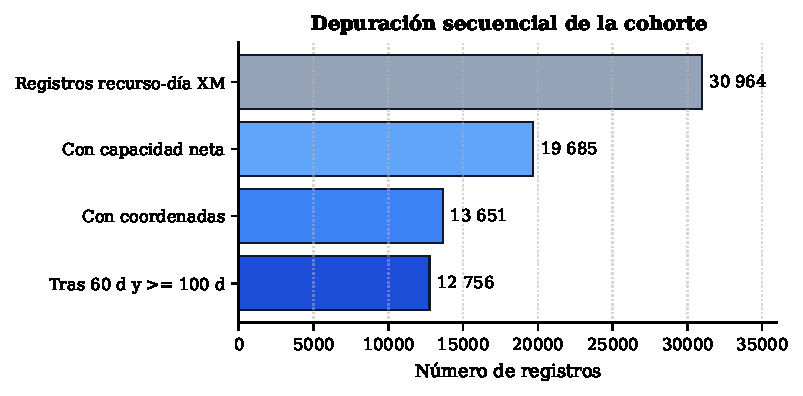
\includegraphics[width=0.86\textwidth]{figures/eda_flujo_cohorte.pdf}\\[0.5em]
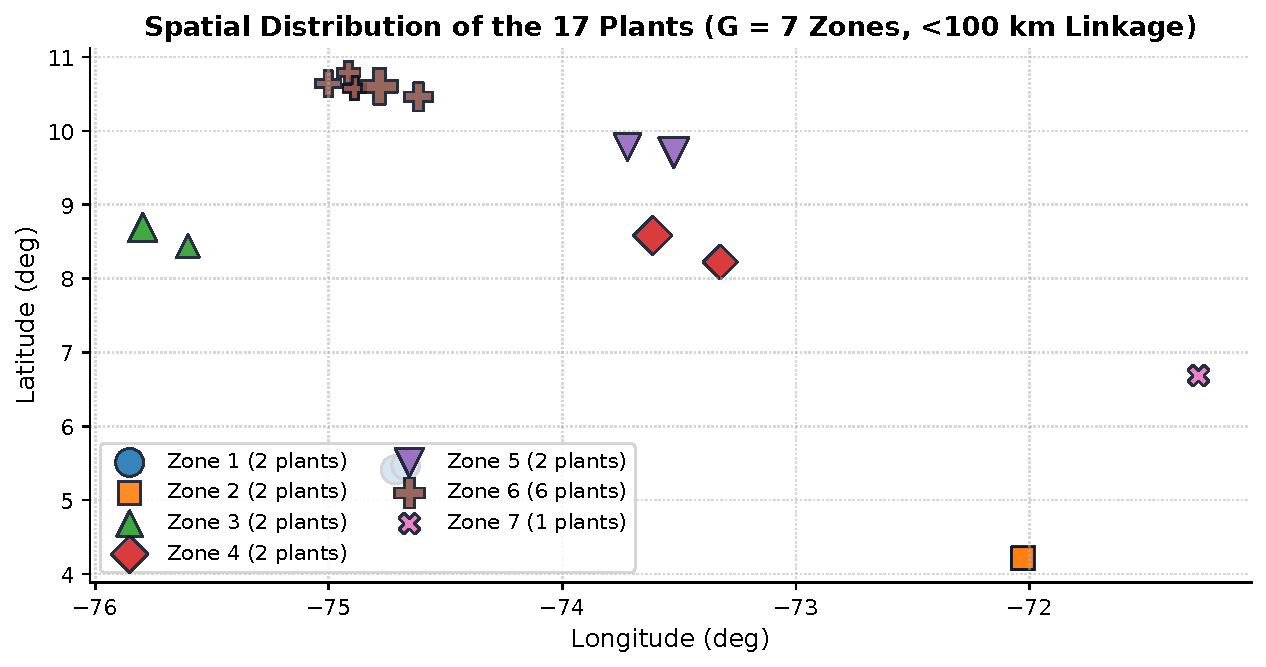
\includegraphics[width=0.86\textwidth]{figures/eda_mapa_plantas.pdf}
\caption{Construcción de la cohorte auditada ($30\,964 \to 12\,756$ filas planta--día en $17$ centrales) y distribución geográfica en $G=7$ grupos espaciales por enlace simple a $<100\text{ km}$.}
\label{fig:cohorte_mapa}
\end{figure}

El análisis exploratorio verifica ausencia de claves duplicadas y revela dos rasgos determinantes para el diseño de SM-CFHR (Figura~\ref{fig:eda_univ} y Apéndice~\ref{ap:eda}): en primer lugar, el factor de capacidad diario presenta media $0{,}248$, mediana $0{,}250$ (rango intercuartílico $0{,}203$--$0{,}295$; máximo $0{,}436$) con una cola izquierda alargada hacia cero que incluye $68$ episodios de rendimiento específico reducido ($\mathrm{cf}\times 24/G_{p,t} < 0{,}3$) asociados a \textit{curtailment}, desconexiones parciales o nubosidad extrema; en segundo lugar, se registran $7$ ampliaciones escalonadas de capacidad neta en $6$ centrales (por ejemplo, \texttt{3HF5} de $90$ a $100$~MW y \texttt{TPUY} de $83$ a $100$~MW), lo que justifica normalizar exclusivamente con la capacidad vigente al origen $C_{i,t}$.

\begin{figure}[!htbp]
\centering
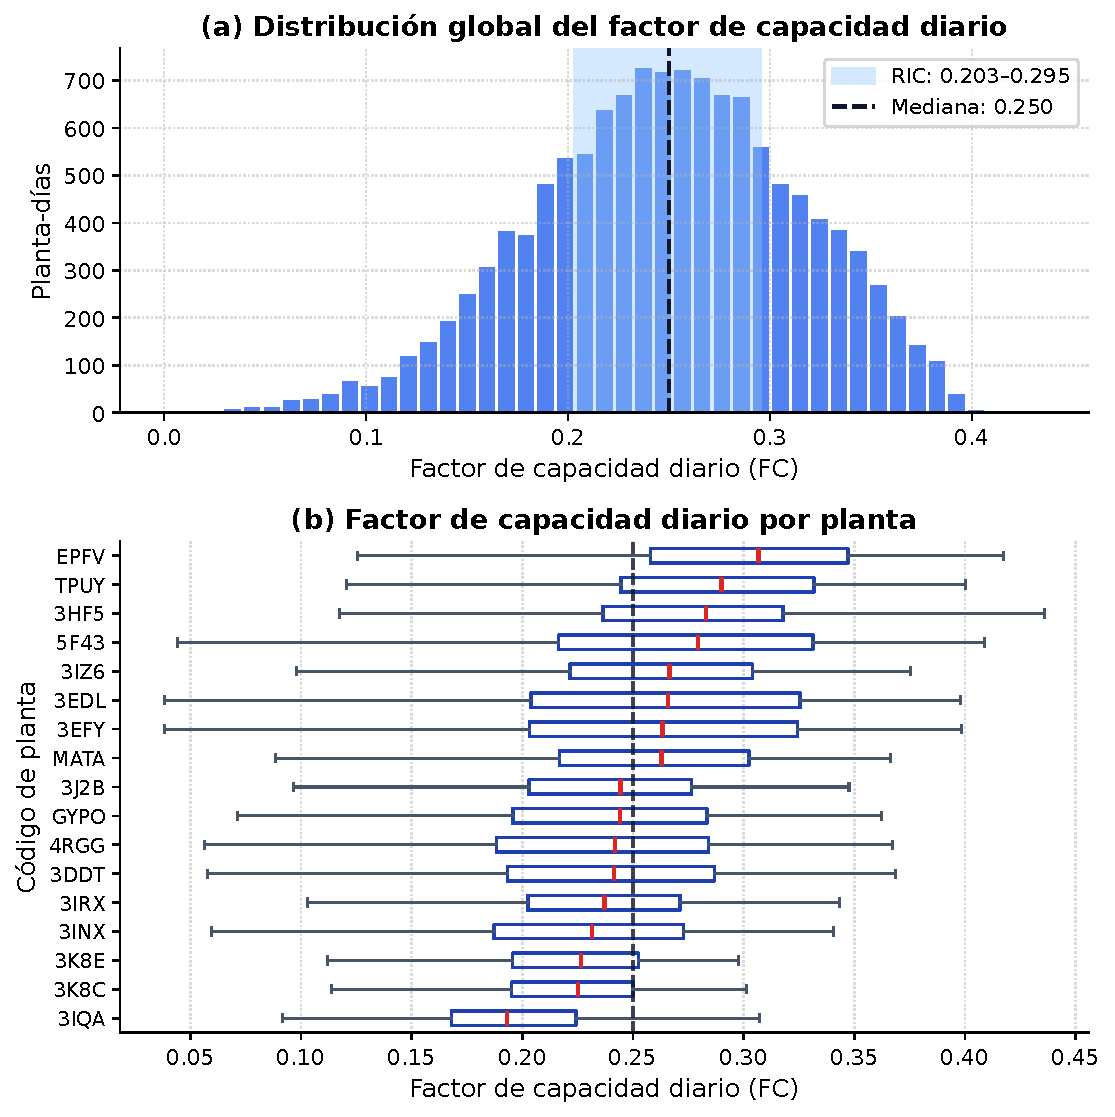
\includegraphics[width=0.49\textwidth]{figures/eda_distribucion_fc.pdf}
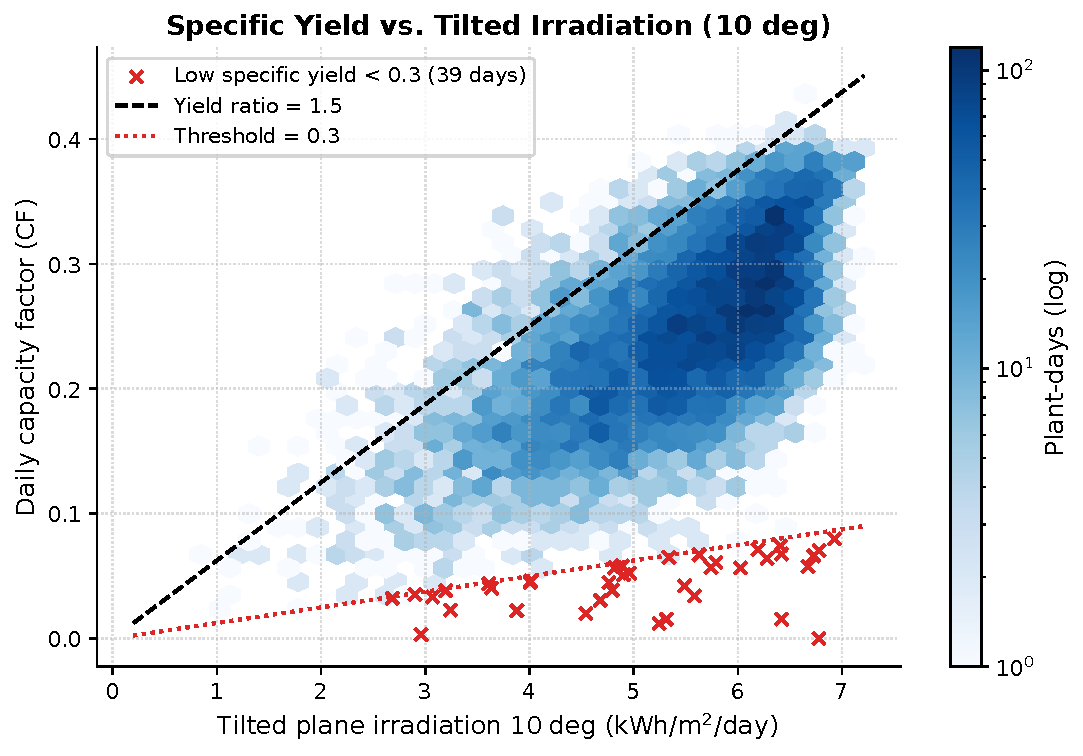
\includegraphics[width=0.49\textwidth]{figures/eda_rendimiento_especifico.pdf}
\caption{Distribución asimétrica del factor de capacidad diario observado (izquierda) y relación frente a la irradiación diaria destacando episodios de bajo rendimiento específico (derecha).}
\label{fig:eda_univ}
\end{figure}

\begin{table}[!htbp]
\caption{Caracterización de las $17$ centrales fotovoltaicas de la cohorte (\texttt{base\_planta\_dia.csv}, ordenado por grupo espacial).}\label{tab:flota17}
\scriptsize
\setlength{\tabcolsep}{3.5pt}
\begin{tabular}{@{}clrrrrrr@{}}
\toprule
Cód. & Planta & Gr. & $n$ total & Cap.\ mín--máx (MW) & Inicio & Fin & Lat / Lon ($^\circ$) \\
\midrule
\texttt{3IRX} & Portón del Sol & 1 & 884 & $102{,}0$--$102{,}0$ & 2024-05-07 & 2026-10-31 & $5{,}41 / -74{,}71$ \\
\texttt{TPUY} & Parque Solar Tepuy & 1 & 812 & $83{,}0$--$100{,}0$ & 2024-08-11 & 2026-10-31 & $5{,}47 / -74{,}67$ \\
\texttt{3EDL} & Bosques Llanos V & 2 & 1\,034 & $17{,}9$--$17{,}9$ & 2024-01-01 & 2026-10-31 & $4{,}21 / -72{,}03$ \\
\texttt{3EFY} & Bosques Llanos IV & 2 & 1\,034 & $19{,}9$--$19{,}9$ & 2024-01-01 & 2026-10-31 & $4{,}22 / -72{,}03$ \\
\texttt{3IZ6} & Parque Solar La Unión & 3 & 805 & $100{,}0$--$102{,}0$ & 2024-08-18 & 2026-10-31 & $8{,}69 / -75{,}80$ \\
\texttt{3J2B} & Solar Planeta Rica & 3 & 868 & $19{,}9$--$19{,}9$ & 2024-06-16 & 2026-10-31 & $8{,}44 / -75{,}60$ \\
\texttt{3IQA} & Sunnorte & 4 & 643 & $35{,}0$--$35{,}0$ & 2025-01-25 & 2026-10-31 & $8{,}22 / -73{,}32$ \\
\texttt{MATA} & La Mata & 4 & 796 & $80{,}0$--$83{,}0$ & 2024-08-26 & 2026-10-31 & $8{,}59 / -73{,}61$ \\
\texttt{3DDT} & Latam Solar La Loma & 5 & 795 & $150{,}0$--$150{,}0$ & 2024-08-23 & 2026-10-31 & $9{,}71 / -73{,}52$ \\
\texttt{EPFV} & El Paso & 5 & 892 & $68{,}0$--$70{,}0$ & 2024-05-22 & 2026-10-31 & $9{,}78 / -73{,}72$ \\
\texttt{3HF5} & Fundación & 6 & 800 & $90{,}0$--$100{,}0$ & 2024-08-21 & 2026-10-31 & $10{,}46 / -74{,}62$ \\
\texttt{3INX} & Caracolí I & 6 & 618 & $50{,}0$--$50{,}0$ & 2025-02-20 & 2026-10-31 & $10{,}64 / -75{,}00$ \\
\texttt{3K8C} & BSB 503 & 6 & 699 & $19{,}9$--$19{,}9$ & 2024-11-25 & 2026-10-31 & $10{,}57 / -74{,}89$ \\
\texttt{3K8E} & BSB 504 & 6 & 698 & $19{,}9$--$19{,}9$ & 2024-11-26 & 2026-10-31 & $10{,}58 / -74{,}89$ \\
\texttt{4RGG} & Parque Solar Baranoa & 6 & 490 & $19{,}9$--$19{,}9$ & 2025-06-29 & 2026-10-31 & $10{,}79 / -74{,}92$ \\
\texttt{GYPO} & Guayepo & 6 & 635 & $370{,}0$--$388{,}0$ & 2025-01-29 & 2026-10-31 & $10{,}61 / -74{,}78$ \\
\texttt{5F43} & Alma II & 7 & 253 & $9{,}8$--$9{,}8$ & 2026-02-21 & 2026-10-31 & $6{,}69 / -71{,}28$ \\
\botrule
\end{tabular}
\end{table}

\subsection{Los 28 escenarios, 22 modelos de referencia y protocolo de validación}

El universo experimental comprende \textbf{28 escenarios oficiales} organizados en cuatro familias (listados en la Tabla~\ref{tab:escenarios28} del Apéndice~\ref{ap:escenarios}):
\begin{enumerate}
    \item \textbf{Horizonte $D+1$ ($4$ escenarios):} regímenes ET e IP $\times$ con meteorología archivada y sin meteorología, evaluados sobre los tres bloques trimestrales $D_1$ (noviembre 2025--enero 2026), $D_2$ (febrero--abril 2026) y $D_3$ (mayo--julio 2026).
    \item \textbf{Recursivo sin clima ($8$ escenarios):} horizontes $H \in \{7,14,21,28\}$ días $\times$ ET e IP, con orígenes contiguos no solapados tras un calentamiento inicial de $90$ días.
    \item \textbf{Directo sin clima ($8$ escenarios):} horizontes $H \in \{7,14,21,28\}$ días $\times$ ET e IP sobre energía acumulada en ventanas completas válidas.
    \item \textbf{Recursivo con clima GEFSv12 ($8$ escenarios):} horizontes $H \in \{7,14,21,28\}$ días $\times$ ET e IP acoplando pronósticos operacionales NOAA GEFSv12 emitidos al origen.
\end{enumerate}

En todos los escenarios se compara contra el inventario oficial congelado de \textbf{22 procedimientos previos}: $9$ estimadores de biblioteca en \texttt{scikit-learn} y \texttt{xgboost} (\texttt{XGBoost}, \texttt{Random Forest}, \texttt{Ridge}, \texttt{SVR}, \texttt{HistGradientBoosting}, \texttt{k-NN}, \texttt{Lasso}, \texttt{BayesianRidge}, \texttt{DecisionTree}), $12$ formulaciones personalizadas del proyecto (\texttt{RLAC}, \texttt{IWLAR}, \texttt{WCFC}, \texttt{ABGPR}, \texttt{HARC}, \texttt{SRMOS}, \texttt{ELAC}, \texttt{KLAC}, \texttt{RARC}, \texttt{RQRF}, \texttt{PDEC}, \texttt{MARB}) y la referencia causal \texttt{Media móvil de 30 días} (\texttt{MM30}). Como se indicó en la introducción, \texttt{CF-BRH} queda explícitamente excluido.

Para garantizar equidad de presupuestos de búsqueda y evitar cualquier sesgo de selección \cite{varma2006bias,cawley2010overfit}, el protocolo pre-registrado distingue dos niveles: \texttt{SM-CFHR-Fixed} ($B=0$ evaluaciones de HPO) constituye la comparación primaria frente a los $22$ modelos de referencia (que emplearon una rejilla acotada de $4$ configuraciones), mientras que \texttt{SM-CFHR-HPO} ($B=25$ evaluaciones TPE) se reporta como análisis secundario. En \texttt{SM-CFHR-HPO}, toda optimización ocurre estrictamente dentro del conjunto de entrenamiento externo de cada pliegue mediante validación cruzada causal anidada de $3$ particiones (Figura~\ref{fig:validacion_anidada}): se impone una brecha causal de embargo de $30$ días en $D+1$ y $t_{\mathrm{end}} \le t_{\mathrm{val}}$ en esquemas directo y recursivo; en régimen ET, cada partición interna mantiene separación espacial estricta excluyendo del entrenamiento interno al grupo espacial validado, descartando cualquier partición que incumpla la separación o los tamaños mínimos ($n_{\mathrm{tr}}\ge 15$, $n_{\mathrm{va}}\ge 5$) en lugar de relajar silenciosamente la restricción espacial. Finalmente, la función \texttt{align\_predictions} exige coincidencia exacta de llaves sin valores faltantes, duplicados ni descartes silenciosos de filas frente a los CSV oficiales de referencia.

\begin{figure}[!htbp]
\centering
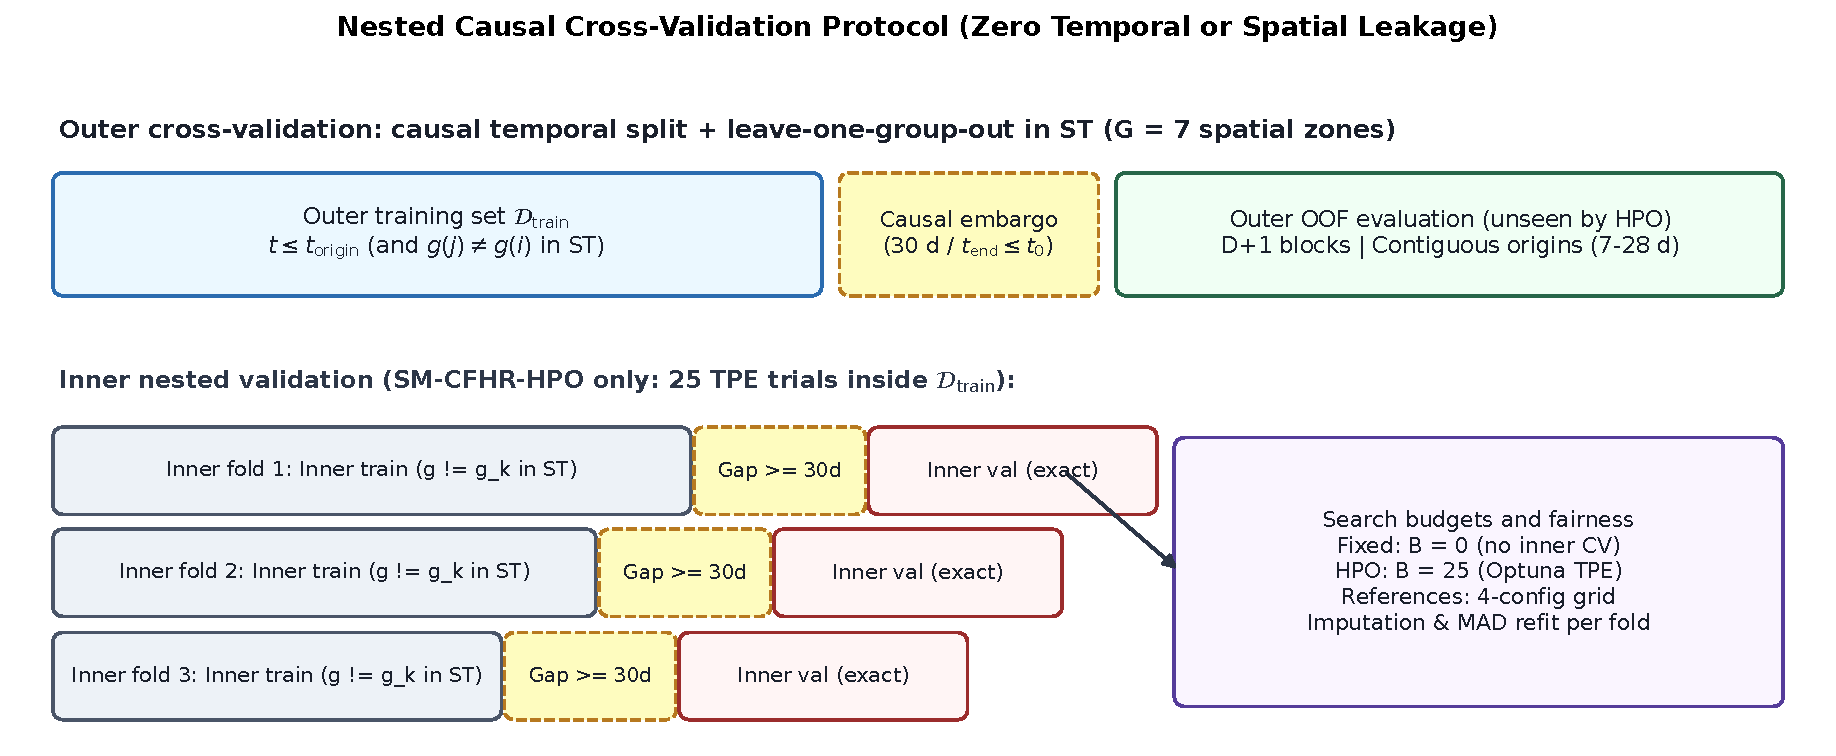
\includegraphics[width=0.98\textwidth]{figures/fig_validacion_anidada.pdf}
\caption{Esquema de validación cruzada causal anidada: separación temporal y espacial externa (\textit{leave-one-group-out} en ET) con brecha de embargo causal de $30$ días y validación interna de $3$ pliegues para TPE HPO.}
\label{fig:validacion_anidada}
\end{figure}

De manera transparente, reiteramos la distinción metodológica entre desarrollo del modelo y evidencia confirmatoria: aunque los parámetros de SM-CFHR se congelaron antes de ejecutar la evaluación OOF definitiva y el código cuenta con auditorías automatizadas anti-fuga, tanto SM-CFHR como los $22$ benchmarks se evaluarán sobre el panel histórico 2024--2026 ya consultado durante la fase exploratoria. Además, no se evalúan conjuntos de datos externos ajenos al dominio solar en esta entrega, quedando dicha modificación de alcance sujeta a validación académica explícita.
